\documentclass[12pt,a4paper]{ctexart}
\usepackage[left=2.6cm,right=2.6cm,top=2.6cm,bottom=2.6cm]{geometry}
\usepackage{graphicx}
\usepackage{booktabs}
\usepackage{array}
\usepackage{longtable}
\usepackage{setspace}
\usepackage{hyperref}
\usepackage{fancyhdr}
\usepackage{titlesec}
\usepackage{caption}
\usepackage{xcolor}
\usepackage{fancyvrb}
\usepackage{enumitem}

\setCJKmainfont[BoldFont=SimHei]{SimSun}
\setCJKmonofont{NSimSun}
\setmonofont{Consolas}
\setlength{\parindent}{2em}
\setlength{\parskip}{0pt}
\setlength{\emergencystretch}{3em}
\linespread{1.28}
\graphicspath{{latex_assets/}}
\hypersetup{colorlinks=true,linkcolor=black,urlcolor=blue}
\pagestyle{fancy}
\fancyhf{}
\fancyfoot[C]{\thepage}
\renewcommand{\headrulewidth}{0pt}
\captionsetup{font=small}

\titleformat{\section}{\zihao{4}\bfseries}{\thesection}{0.6em}{}
\titleformat{\subsection}{\zihao{-4}\bfseries}{\thesubsection}{0.6em}{}
\titleformat{\subsubsection}{\zihao{5}\bfseries}{\thesubsubsection}{0.6em}{}

\begin{document}

\begin{titlepage}
    \centering
    \vspace*{2.2cm}
    {\zihao{2}\bfseries 《数字化集成控制系统》期末实验报告\par}
    \vspace{2.8cm}
    {\zihao{4}班级：强基班 \quad 姓名：匿名 \quad 学号：\par}
    \vspace{1.1cm}
    {\zihao{4}课程名称：数字化集成控制系统\par}
    \vspace{1.1cm}
    {\zihao{4}报告内容：定位跑、折返跑、跨栏跑、位置 PID、双闭环 PID\par}
    \vfill
    {\zihao{-4}\today\par}
\end{titlepage}

\tableofcontents
\clearpage

\section*{摘要与关键词}
\addcontentsline{toc}{section}{摘要与关键词}

本报告围绕数字化集成控制系统课程中的五个实验题展开，结合现有 STL 程序与说明书资料，对从基础顺序控制到闭环 PID 控制的实现过程进行了系统整理。报告首先分析实验任务对定位、折返、分段变速和参数交互的要求，然后给出基于 S7-200 PLC、编码器、HMI、变频器和电机执行机构的总体设计方案；在此基础上，对高速计数、位置反馈、PID 调节及双闭环控制原理进行说明，并逐项分析定位跑、折返跑、跨栏跑、位置 PID 定位跑以及位置/速度双闭环 PID 折返跑的实现逻辑、关键变量和控制特点。实验结果表明，系统能够完成课程要求中的多模式运动控制任务，其中基础程序验证了计数器与顺序逻辑的可行性，进阶程序则体现了闭环反馈在抑制超调、提高定位稳定性方面的优势。为了便于后续排版和复核，完整 STL 源程序统一整理于附录。

\noindent\textbf{关键词：}S7-200 PLC；高速计数；定位控制；PID；数字化集成控制系统

\clearpage
\section{系统总体方案设计}

\subsection{系统需求分析}
本次实验需要在同一套电机控制装置上完成五个递进式任务：定位跑要求系统在给定圈数后准确停止；折返跑要求系统在多个位置点之间切换方向；跨栏跑要求系统在全程运行过程中按照预设位置切换速度；位置 PID 定位跑要求系统利用编码器反馈实现更平滑、更稳定的闭环到位；双闭环 PID 折返跑则进一步要求系统同时处理位置和速度两个维度的动态误差。由此可以看出，系统必须同时具备顺序控制、位置检测、状态切换、速度调节以及参数扩展能力。

结合当前素材，系统需求可以归纳为三类。其一是运动控制需求，即在不同模式下完成定距运行、往返切换、分段变速和终点停机；其二是信号与交互需求，即通过 HMI 实现参数输入，通过编码器完成位置反馈，通过 PLC 输出方向和速度控制信号；其三是性能需求，即程序结构清晰、运行稳定、能够为后续 PID 参数整定和人机交互扩展留下空间。

\subsection{系统硬件与软件架构设计}

\subsubsection{硬件架构设计}
本系统以 S7-200 PLC 为核心控制单元，配合 HMI 触摸屏、增量式编码器、FRS520SE 变频器、电机执行机构以及电源模块构成完整控制链路。PLC 负责读取编码器脉冲、解析模式参数、执行顺序逻辑和 PID 运算；编码器通过 A/B 相信号把电机实际位置反馈给 PLC 的高速计数输入；HMI 提供参数输入和状态显示；变频器接收方向与速度指令后驱动电机运行。硬件结构如图 \ref{fig:hardware} 所示。

\begin{figure}[htbp]
    \centering
    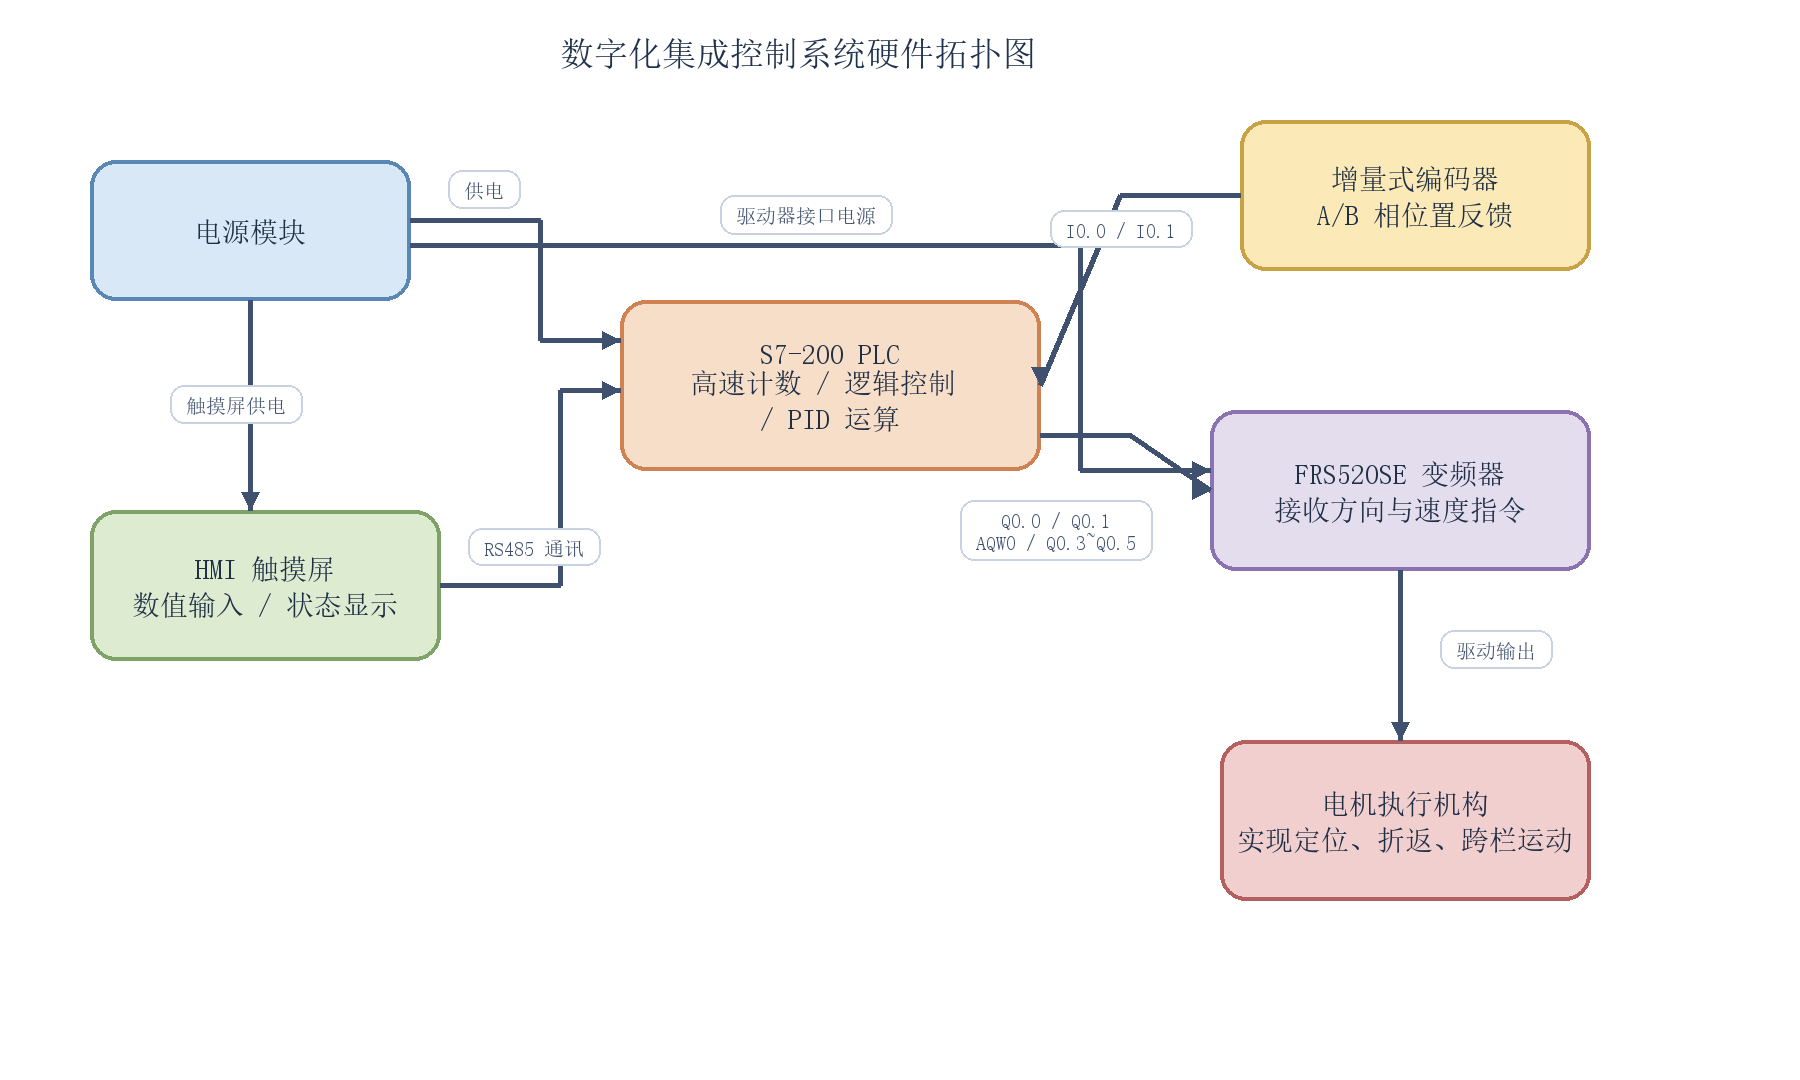
\includegraphics[width=0.95\textwidth]{hardware_topology.png}
    \caption{系统硬件拓扑图}
    \label{fig:hardware}
\end{figure}

从现有程序和说明书可知，编码器主要接入 I0.0/I0.1，高速计数器用于记录电机位置；Q0.0、Q0.1 负责正反转控制；Q0.3、Q0.4、Q0.5 用于速度档位选择；在位置 PID 实验中，AQW0 被用于输出连续模拟量，从而实现更细腻的速度调节。这样的硬件分工为后续从开环逻辑到闭环调节的升级提供了清晰基础。

\subsubsection{软件架构设计}
软件层面采用主程序加子程序的分层组织方式。主程序负责初始化、读取参数、模式判断和结束判定；各个实验模式则分别封装为独立的控制逻辑单元。这样既能共享基础资源，又便于逐题调试和性能对比。总体流程如图 \ref{fig:software} 所示。

\begin{figure}[htbp]
    \centering
    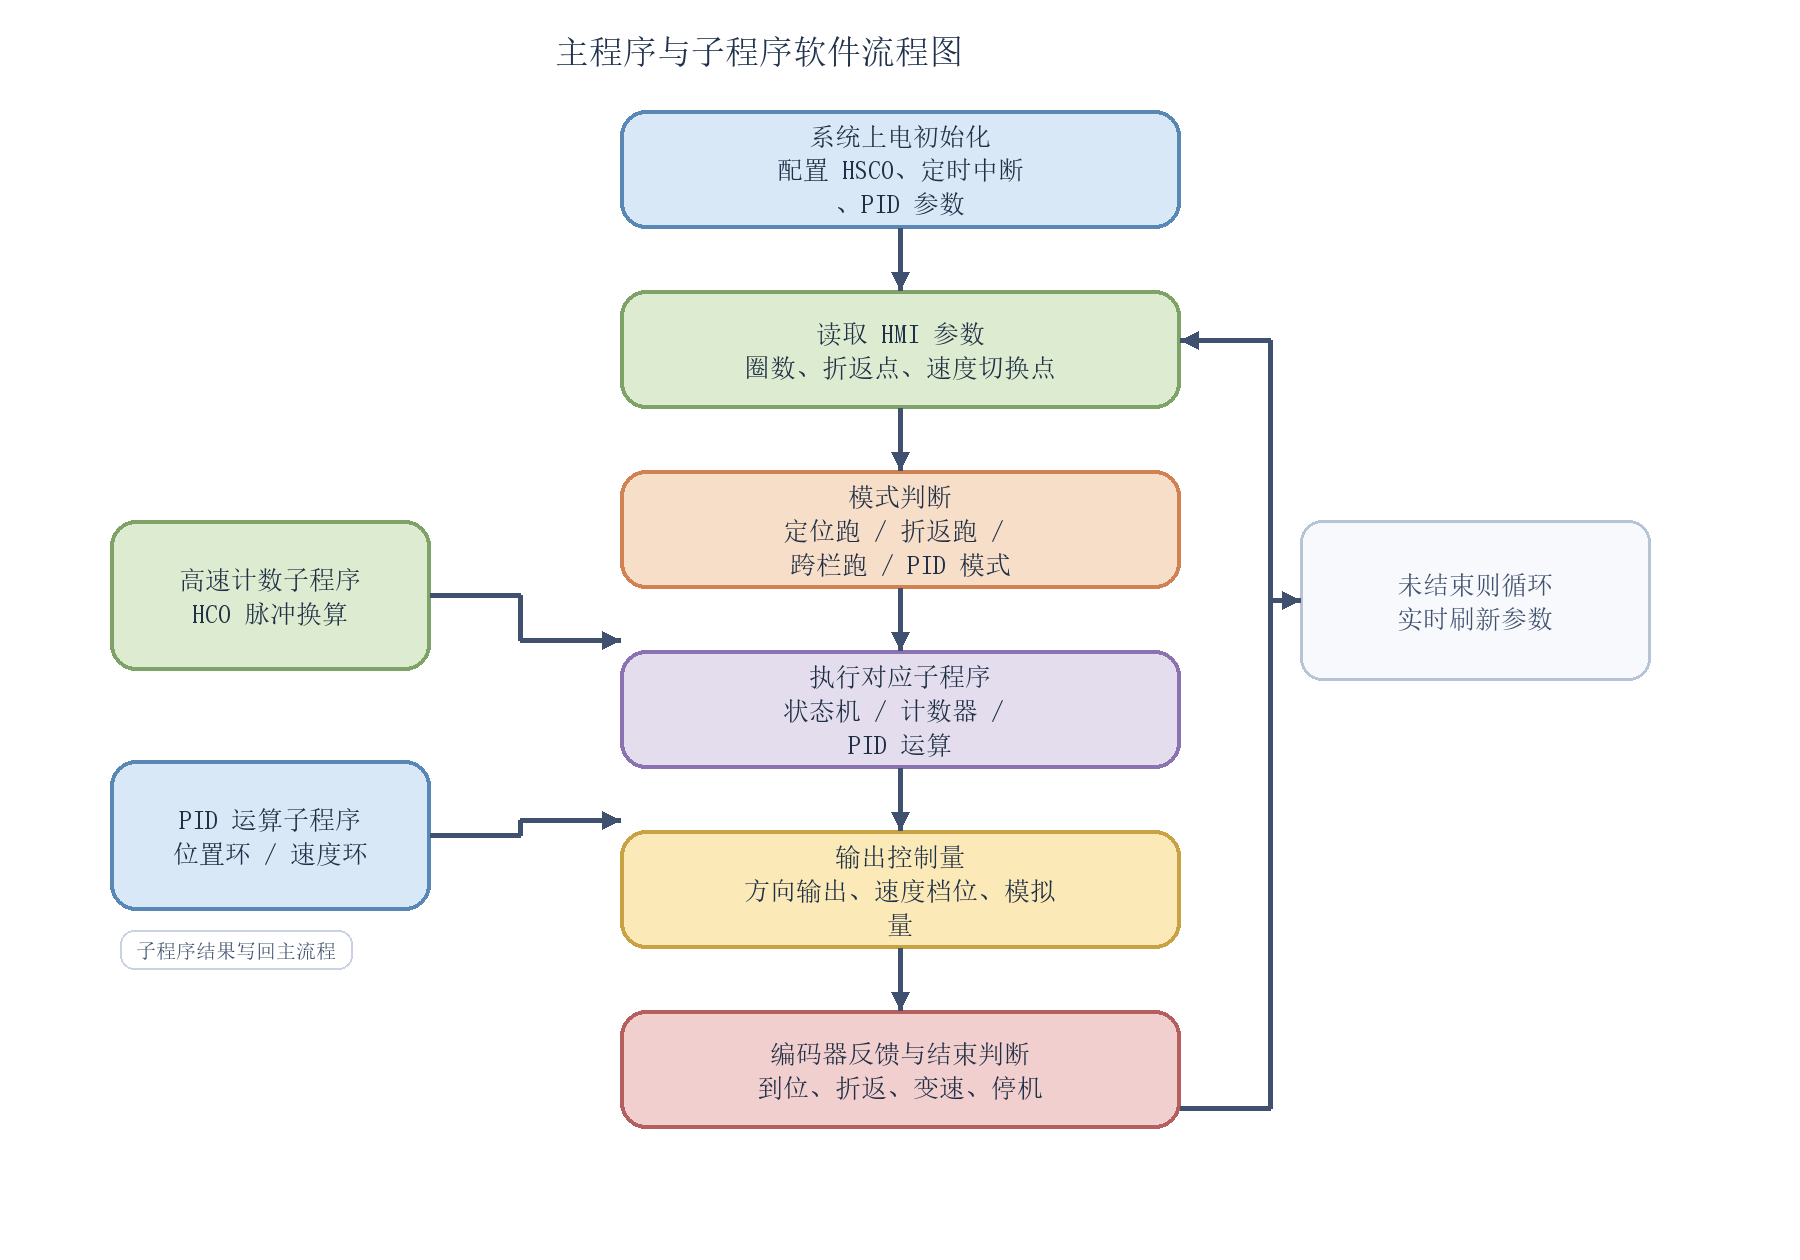
\includegraphics[width=0.92\textwidth]{software_flow.png}
    \caption{主程序与子程序软件流程图}
    \label{fig:software}
\end{figure}

程序运行时，系统首先完成 HSC0、定时中断和 PID 参数表初始化，然后读取 HMI 参数或实验预设值，随后根据运行模式调用对应子程序。执行过程中，编码器反馈不断更新当前位置或速度估计值，为变速判断、折返点判断和闭环运算提供依据；若系统尚未结束，则继续刷新参数并执行下一轮运算。

\clearpage
\section{基础控制原理与概念}

\subsection{电机运动控制基础概念}

\subsubsection{定位控制与闭环控制}
定位控制的基本目标是在给定距离或给定脉冲数附近停止电机。对于课程中的基础实验，采用“计数达到阈值即停机”的方法即可完成任务，这属于典型的顺序逻辑控制；而闭环控制则要求系统持续比较目标值与反馈值，根据偏差实时修正输出，因此更适合高精度、低超调的定位任务。

\subsubsection{增量式编码器工作原理}
增量式编码器通过 A/B 两相信号输出脉冲，PLC 可以依据脉冲数量判断位移，依据相位关系判断转向。在本实验中，编码器脉冲既可用于统计圈数，也可用于构造位置反馈和测速量，是实现定位跑、折返跑和 PID 控制的关键基础。

\subsubsection{PLC 高速计数器与 HMI 交互原理}
普通扫描方式难以稳定采集高速脉冲，因此需要借助 S7-200 的高速计数器功能。现有程序中通过 SMB37、SMD38 等寄存器完成 HSC0 的定义、清零和更新，保证位置反馈的可靠性。与此同时，HMI 的数值输入控件为后续圈数、折返点和变速点参数化提供了界面基础，使系统具备从固定设定向在线可调扩展的能力。

\subsection{PID 控制理论基础}
PID 控制由比例、积分和微分三部分组成。比例环节决定系统对偏差的即时响应强度，积分环节用于消除稳态误差，微分环节则通过感知偏差变化趋势来抑制过冲和振荡。在位置 PID 实验中，程序通过标准化的位置偏差驱动模拟量输出，并在接近终点时使用刹车死区强化稳定性；在双闭环 PID 实验中，位置环负责给出目标速度，速度环再根据测速结果对实际输出进行修正，从而实现更平稳的往返定位。

\section{控制方案设计}
本节结合五份 STL 程序分析每个实验题的实现思路和控制特点。为控制正文篇幅，完整源程序统一置于附录，正文只保留关键结构和结论。

\subsection{定位跑控制方案与理论要点}
定位跑程序用于完成电机运行三圈后的自动停车。程序首先在首次扫描时初始化 HSC0，将目标值设置为 1200 脉冲；启动时置位运行标志与方向标志，并将当前计数清零。运行期间，PLC 持续把 HC0 当前值搬移到数据寄存器，当当前位置达到目标脉冲时置位到位标志，随后复位运行和方向输出，实现自动停机。完整 STL 程序见附录 A。

该方案优点在于结构简单、调试直接，适合验证编码器反馈与计数功能是否正确；不足之处在于停机动作更接近开关控制，当速度较高或惯性较大时，终点附近的稳定性有限，这也是后续引入 PID 闭环的主要原因。

\subsection{折返跑控制方案与理论要点}
折返跑程序以计数器和状态分段为核心。程序先用计数器记录脉冲，再借助多个中间状态判断不同区段是否结束，通过控制 Q0.0、Q0.1 等方向输出实现往返切换。其核心思想是把整个运行过程拆解为多个有边界条件的动作段，每到一个折返点就切换到下一段控制逻辑。完整 STL 程序见附录 B。

与定位跑相比，折返跑不再只关注终点，而是要求系统能够在多个节点间可靠切换方向，因此对状态机的设计和条件判断的准确性提出了更高要求。这种思路为后续双闭环 PID 折返跑中的状态管理提供了实践基础。

\subsection{跨栏跑控制方案与理论要点}
跨栏跑程序围绕“全程七圈、分段变速”展开。现有代码利用 C0 记录基本圈数，再通过 C1、C2、C3、C4 构造多个位置节点，以 M0.0 作为总运行标志控制正转输出，并根据不同区间切换 Q0.2、Q0.3、Q0.4 三档速度输出。这样系统即可在起始段、中间段和后段分别采用不同转速，完成分段变速任务。完整 STL 程序见附录 C。

该实验的关键在于将“位置判断”与“速度切换”结合起来，使程序从单一终点判断扩展为多点事件响应。后续若结合 HMI 把三个中间位置开放为可输入参数，则跨栏跑可以进一步发展为更接近工程应用的配方化运行模式。

\subsection{其他选做题目}

\subsubsection{位置 PID 定位跑}
位置 PID 程序在上电时完成 HSC0 与 PID 参数初始化，将目标位置设定为 1185 脉冲，并把当前计数标准化为 0 到 1 的过程变量。PLC 调用原生 PID 指令后，将输出结果换算为模拟量 AQW0，用于控制变频器速度；当位置接近目标值时，程序会立即切断运行信号并把模拟量降为 0，形成终点刹车区，从而避免持续振荡。完整 STL 程序见附录 D。

相对于基础定位跑，位置 PID 定位跑能够在接近终点时主动减速，提高停车的平稳性和精度。该实验的实现重点集中在参数归一化、终点死区设计和超调抑制策略上，因此更能体现闭环控制相对于基础顺序逻辑的优势。

\subsubsection{位置/速度双闭环 PID 折返跑}
双闭环 PID 程序在首次扫描时完成高速计数器、中断参数、位置历史量与速度环积分器初始化，并利用 VW100 构建状态机。程序启动后先执行正向三圈，再回到零点，最后再次正向到终点。位置外环根据当前位置误差给出目标速度，速度内环根据测速结果修正输出，因此系统能够同时兼顾响应速度和最终到位稳定性。完整 STL 程序见附录 E。

双闭环结构把“跑多远”和“跑多快”分开处理：位置环决定应当以怎样的速度逼近目标，速度环负责使实际输出跟随目标速度。与单环位置控制相比，双闭环控制在折返运动这类动态变化较大的任务中更容易取得平稳和精确的综合效果。

\section{总结与展望}
通过本次实验可以看到，数字化集成控制系统的训练路径非常清晰：先用计数器和顺序逻辑完成基础运动任务，再逐步引入位置反馈和 PID 算法实现更高水平的控制效果。定位跑验证了高速计数器的基本使用；折返跑和跨栏跑体现了多阶段逻辑组织的重要性；位置 PID 和双闭环 PID 则展示了反馈控制在提高定位品质方面的明显优势。

在本次整理中，除说明书资料外，还参考了若干公开的 GitHub PLC 学习项目，用于交叉验证顺序控制组织方式、梯形图/结构化文本的表达习惯，以及典型 PLC 任务在教学场景下的拆解方式。这些开源资料主要作为编程思路的辅助来源，而非本实验程序的直接替代。后续若继续完善系统，可将更多运行参数开放给 HMI，增加报警与故障自检逻辑，并对 PID 参数整定提供更直观的可视化界面。

\section*{参考文献}
\addcontentsline{toc}{section}{参考文献}

\begin{sloppypar}
\small
\begin{enumerate}[label={[\arabic*]}]
    \item 西门子（中国）有限公司. S7-200 可编程控制器系统手册[Z]. 2005.
    \item Siemens AG. TP177A/TP177B/OP177B Operating Instructions[Z].
    \item FRS520SE 变频器说明书[Z].
    \item Krishnaelectrovoltz. Sequencing-using-PLC-Logic[EB/OL]. GitHub, 顺序控制与 PLC 教学示例仓库. \url{https://github.com/Krishnaelectrovoltz/Sequencing-using-PLC-Logic}. 访问日期：2026-04-19.
    \item LeandroDQuevedo. plc-study-cases[EB/OL]. GitHub, 基于 IEC 61131-3 的 Ladder 与 Structured Text 示例项目. \url{https://github.com/LeandroDQuevedo/plc-study-cases}. 访问日期：2026-04-19.
    \item sidneyhori. ladder-logic-simulator[EB/OL]. GitHub, 用于查看与复核 PLC 梯形图的交互式样例程序. \url{https://github.com/sidneyhori/ladder-logic-simulator}. 访问日期：2026-04-19.
\end{enumerate}
\normalsize
\end{sloppypar}

\clearpage
\appendix
\section{定位跑 STL 程序}
\VerbatimInput[fontsize=\scriptsize,baselinestretch=0.92,frame=single,numbers=left,numbersep=6pt]{latex_assets/code/dingweipao.txt}

\clearpage
\section{折返跑 STL 程序}
\VerbatimInput[fontsize=\scriptsize,baselinestretch=0.92,frame=single,numbers=left,numbersep=6pt]{latex_assets/code/zhefanpao.txt}

\clearpage
\section{跨栏跑 STL 程序}
\VerbatimInput[fontsize=\scriptsize,baselinestretch=0.92,frame=single,numbers=left,numbersep=6pt]{latex_assets/code/kualanpao.txt}

\clearpage
\section{位置 PID STL 程序}
\VerbatimInput[fontsize=\scriptsize,baselinestretch=0.92,frame=single,numbers=left,numbersep=6pt]{latex_assets/code/position_pid.txt}

\clearpage
\section{双闭环 PID STL 程序}
\VerbatimInput[fontsize=\scriptsize,baselinestretch=0.92,frame=single,numbers=left,numbersep=6pt]{latex_assets/code/dual_pid.txt}

\end{document}
